\section{共形映射}

See Dennis Zill. Appendex III for \underline{Table of Conformal Mappings}

\begin{figure}[H]
\centering
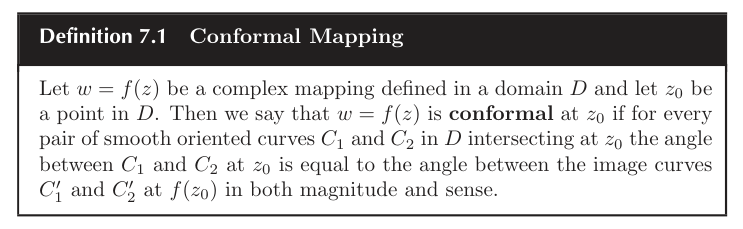
\includegraphics[width=\textwidth]{共形映射-2025051501.png}
% \caption{}
\label{}
\end{figure}
Some examples of conformal mapping:

\begin{enumerate}
	\item Translations: $f(z) = z + b$, where $b$ is a complex number.
	\item Rotations: $f(z) = e^{i\phi} z$, where $\phi$ is a real number.
	\item Dilations (or scalings): $f(z) = rz$, where $r > 0$ is a real number.
	\item Inversion: $f(z) = 1/z$, $z \neq 0$.
	\item Linear transformations: $f(z) = az + b$, where $a, b$ are complex numbers and $a \neq 0$.
	\item Möbius transformations (or linear fractional transformations): $f(z) = \frac{az + b}{cz + d}$, where $a, b, c, d$ are complex numbers and $ad - bc \neq 0$.
\end{enumerate}

\begin{figure}[H]
\centering
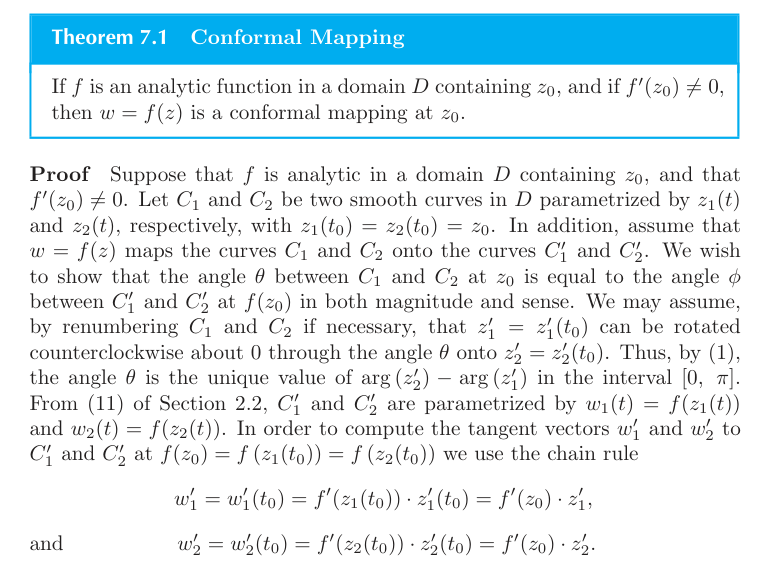
\includegraphics[width=\textwidth]{1-共形映射-2025051501.png}
% \caption{}
\label{}
\end{figure}
\begin{figure}[H]
\centering
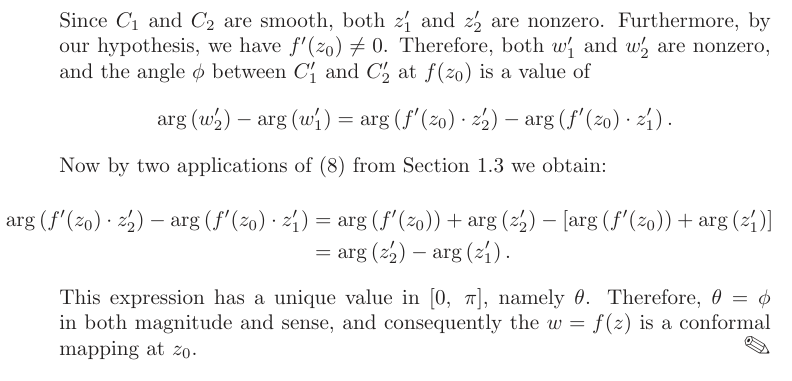
\includegraphics[width=\textwidth]{2-共形映射-2025051501.png}
% \caption{}
\label{}
\end{figure}

\begin{definition}[Simply Connected Domain]
A domain $D$ is \textbf{simply connected} if it is connected and every closed curve in $D$ can be continuously deformed to a point in $D$.
\end{definition}
Then we introduce the Riemann Mapping Theorem:
\begin{figure}[H]
\centering
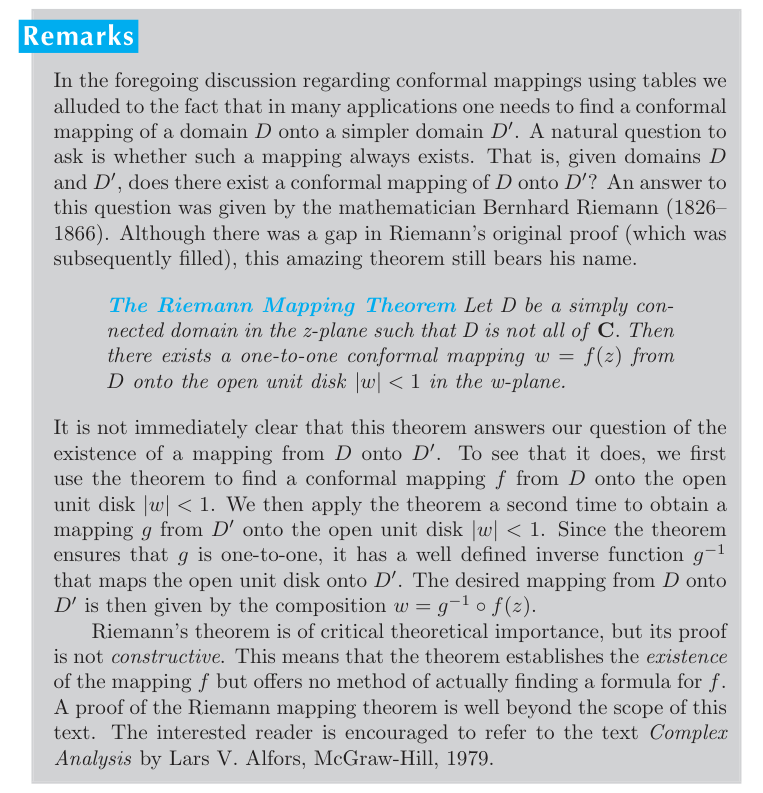
\includegraphics[width=\textwidth]{3-共形映射-2025051501.png}
% \caption{}
\label{}
\end{figure}

\begin{figure}[H]
\centering
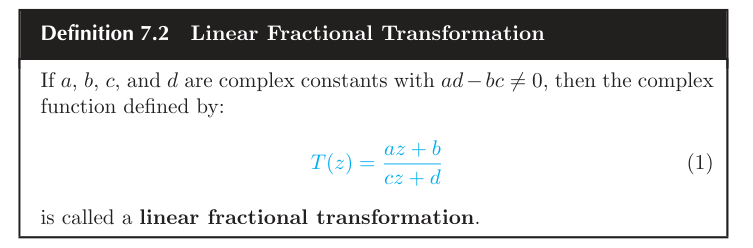
\includegraphics[width=\textwidth]{4-共形映射-2025051501.png}
% \caption{}
\label{}
\end{figure}

Linear fractional transformations are also called \textbf{Möbius transformations} or \textbf{bilinear transformations}.
\begin{figure}[H]
\centering
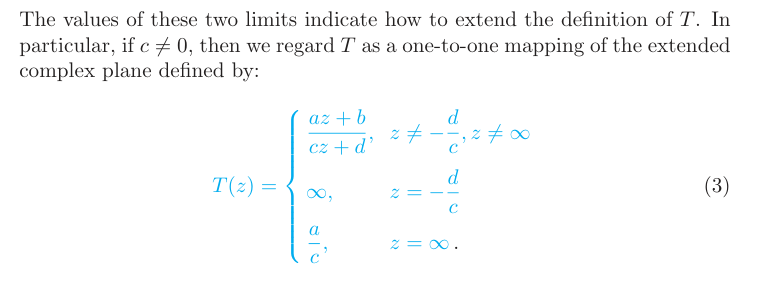
\includegraphics[width=\textwidth]{5-共形映射-2025051501.png}
% \caption{}
\label{}
\end{figure}

\begin{figure}[H]
\centering
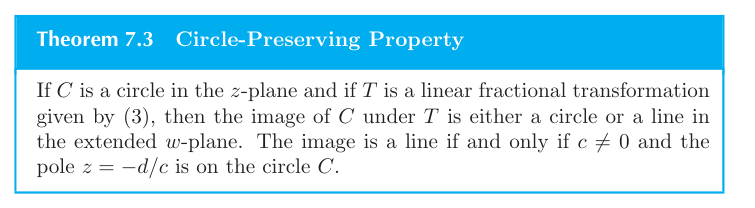
\includegraphics[width=\textwidth]{6-共形映射-2025051501.png}
% \caption{}
\label{}
\end{figure}

\begin{figure}[H]
\centering
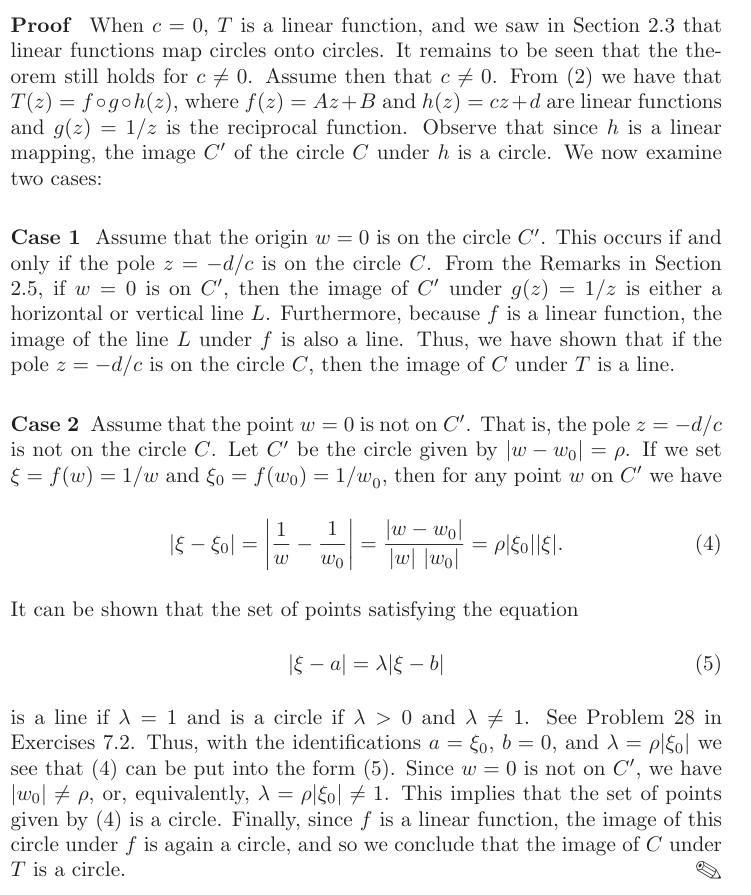
\includegraphics[width=\textwidth]{7-共形映射-2025051501.png}
% \caption{}
\label{}
\end{figure}

\subsection{Linear Fractional Transformations as Matrices}

\begin{figure}[H]
\centering
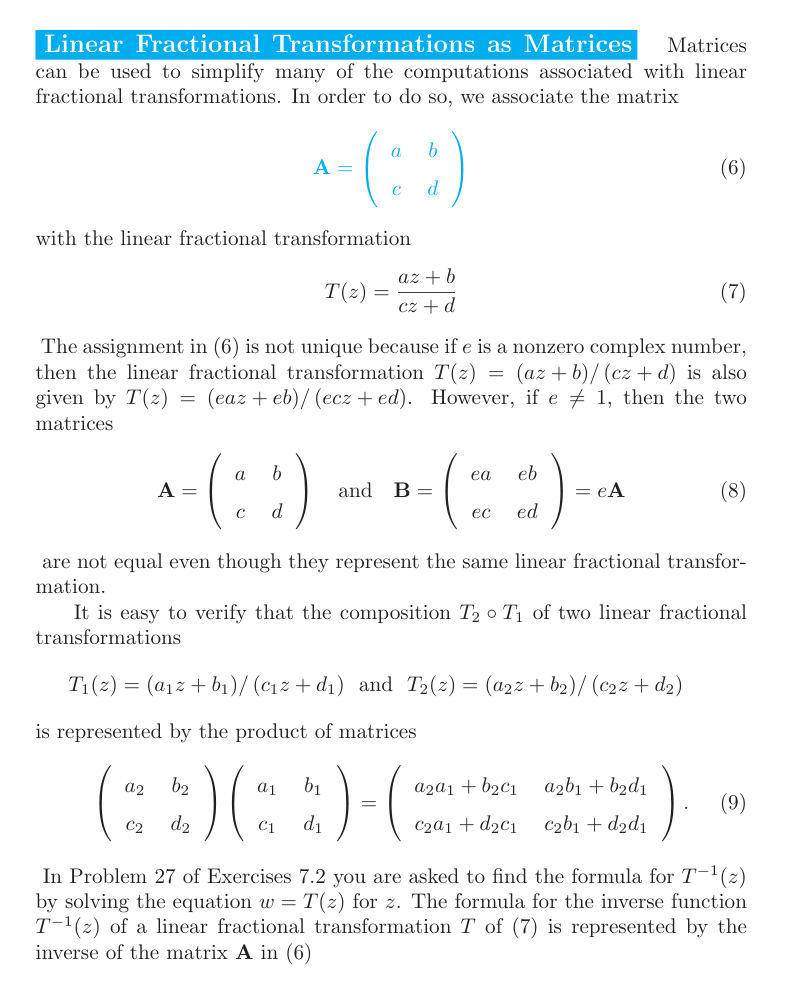
\includegraphics[width=\textwidth]{8-共形映射-2025051501.png}
% \caption{}
\label{}
\end{figure}
\begin{figure}[H]
\centering
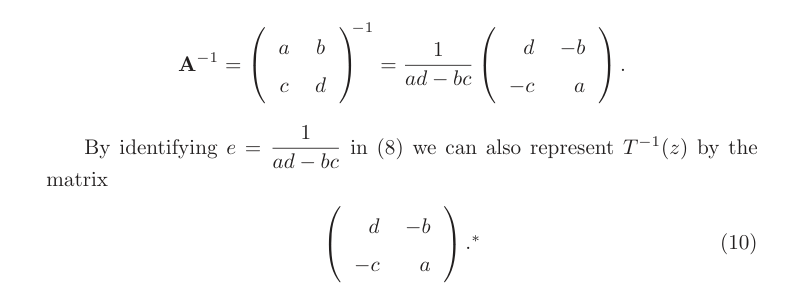
\includegraphics[width=\textwidth]{9-共形映射-2025051501.png}
% \caption{}
\label{}
\end{figure}
This matrix is called the adjoint matrix of $A$.

\begin{figure}[H]
\centering
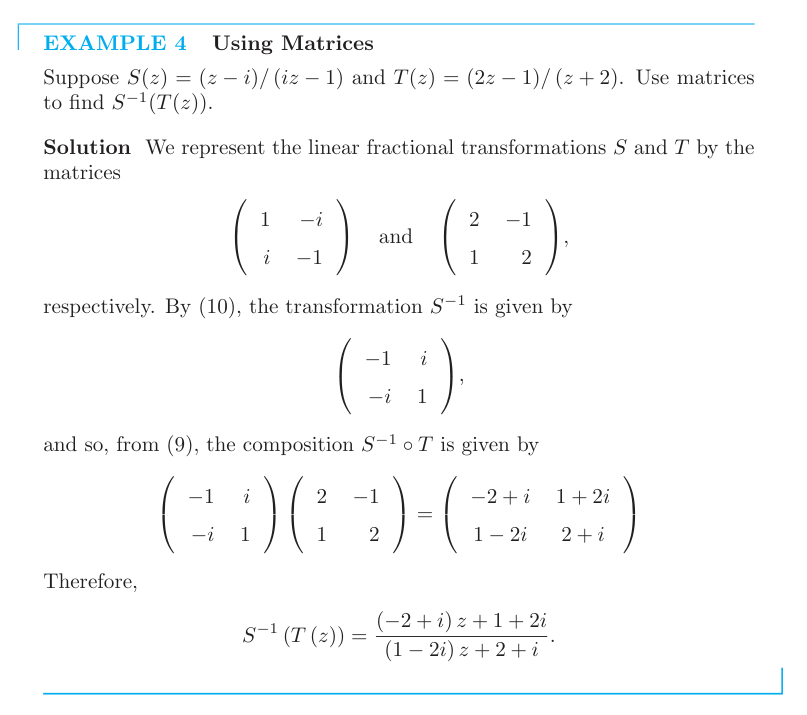
\includegraphics[width=\textwidth]{10-共形映射-2025051501.png}
% \caption{}
\label{}
\end{figure}

\subsection{Cross-ratio}

\begin{figure}[H]
\centering
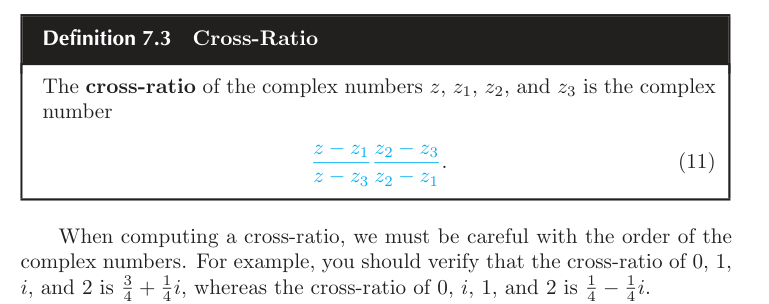
\includegraphics[width=\textwidth]{11-共形映射-2025051501.png}
% \caption{}
\label{}
\end{figure}
\begin{figure}[H]
\centering
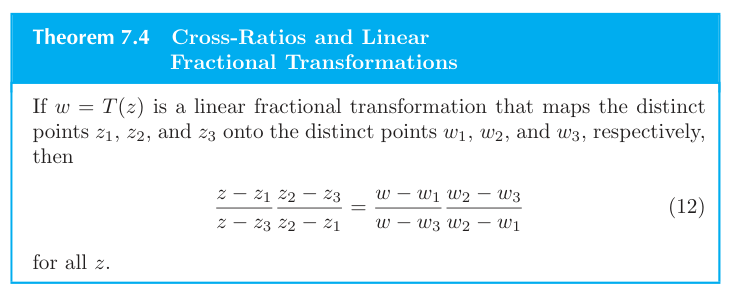
\includegraphics[width=\textwidth]{12-共形映射-2025051501.png}
% \caption{}
\label{}
\end{figure}

\subsubsection{Constructing a Linear Fractional Transform mapping given points to given points}

\begin{figure}[H]
\centering
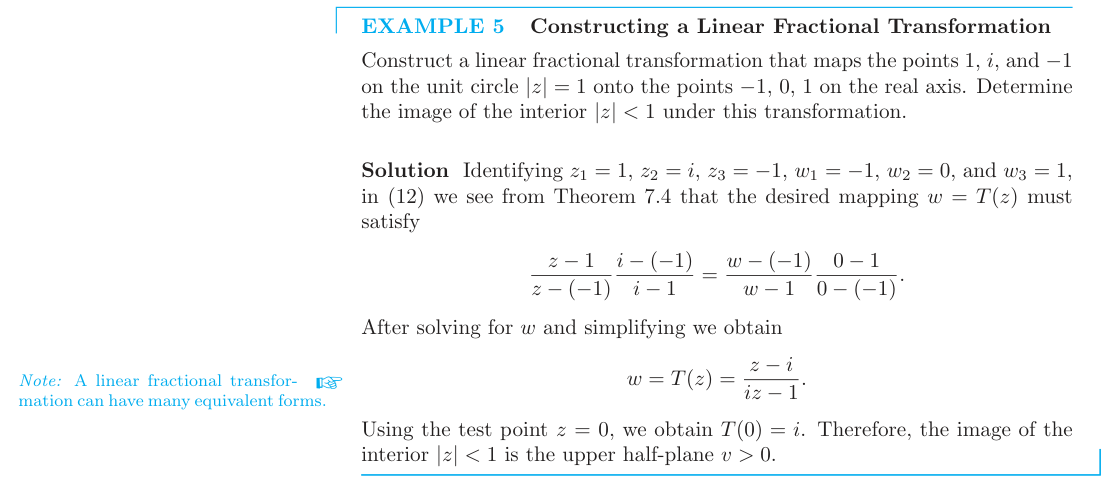
\includegraphics[width=\textwidth]{14-共形映射-2025051501.png}
% \caption{}
\label{}
\end{figure}
\begin{figure}[H]
\centering
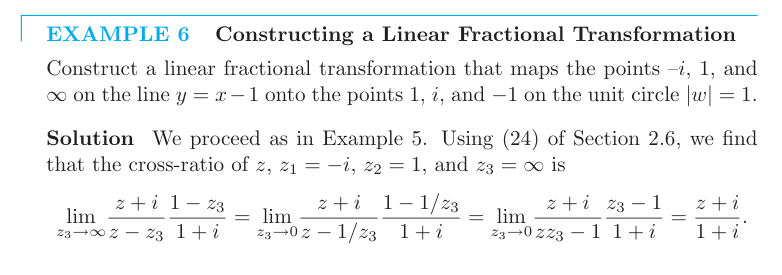
\includegraphics[width=\textwidth]{15-共形映射-2025051501.png}
% \caption{}
\label{}
\end{figure}
\begin{figure}[H]
\centering
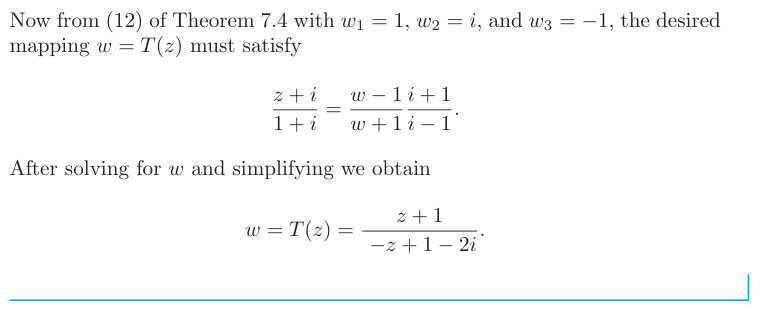
\includegraphics[width=\textwidth]{16-共形映射-2025051501.png}
% \caption{}
\label{}
\end{figure}

\subsection{Schwarz-Christoffel Transformations}

The motivation is from $w=f(z)=(z-x_1)^{\alpha/\pi}$ with $f'(z)=\frac{\alpha}{\pi}(z-x_1)^{(\alpha/\pi)-1}$.

\begin{figure}[H]
\centering
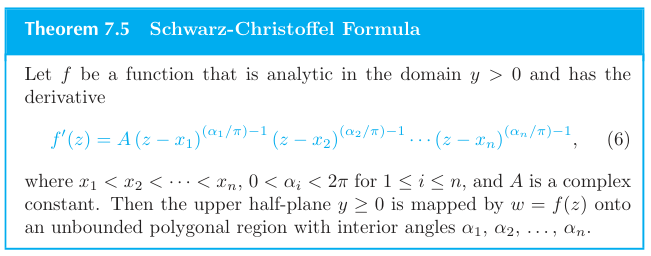
\includegraphics[width=\textwidth]{共形映射-2025061000.png}
% \caption{}
\label{}
\end{figure}
\begin{figure}[H]
\centering
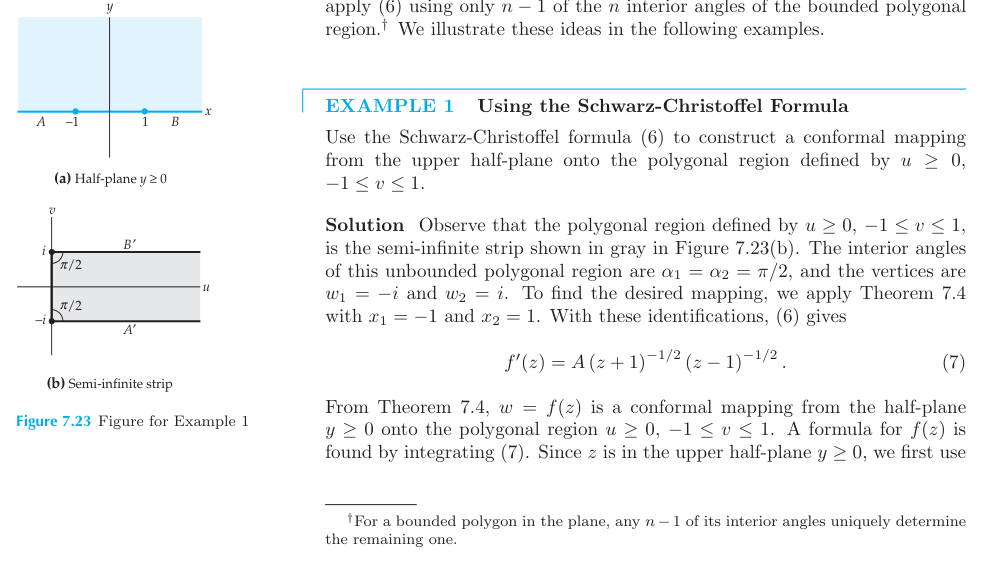
\includegraphics[width=\textwidth]{1-共形映射-2025061000.png}
% \caption{}
\label{}
\end{figure}
\begin{figure}[H]
\centering
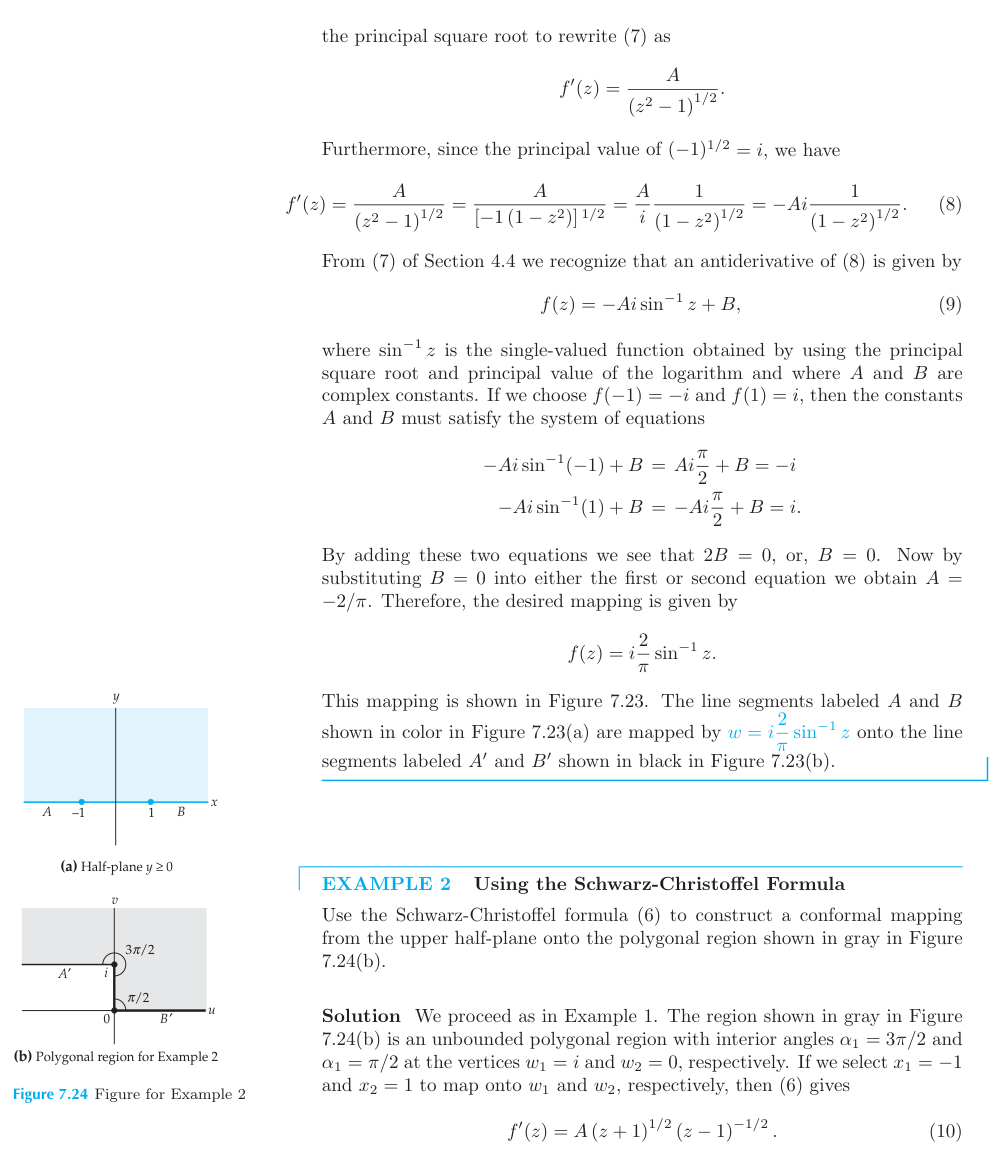
\includegraphics[width=\textwidth]{3-共形映射-2025061000.png}
% \caption{}
\label{}
\end{figure}
\begin{figure}[H]
\centering
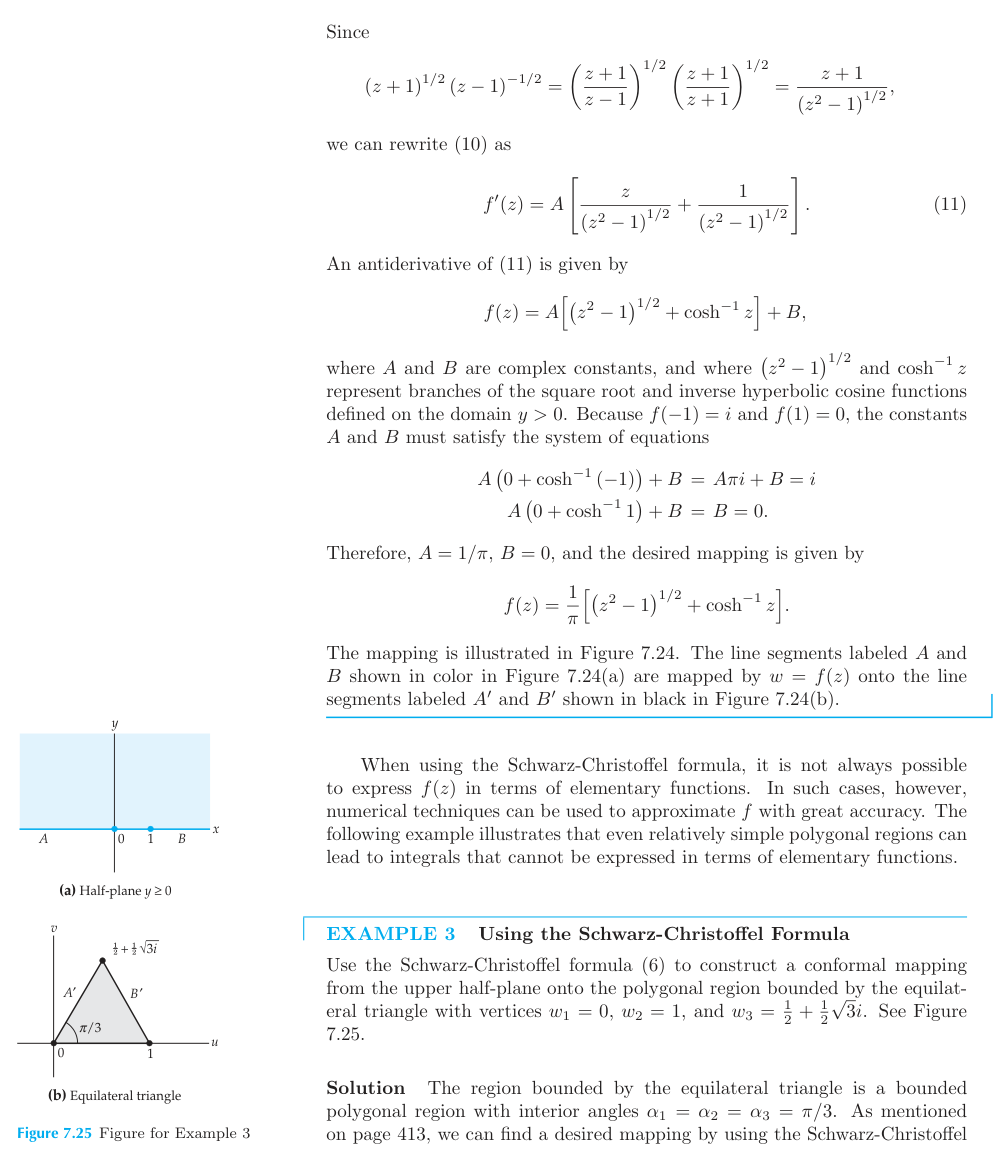
\includegraphics[width=\textwidth]{4-共形映射-2025061000.png}
% \caption{}
\label{}
\end{figure}
\begin{figure}[H]
\centering
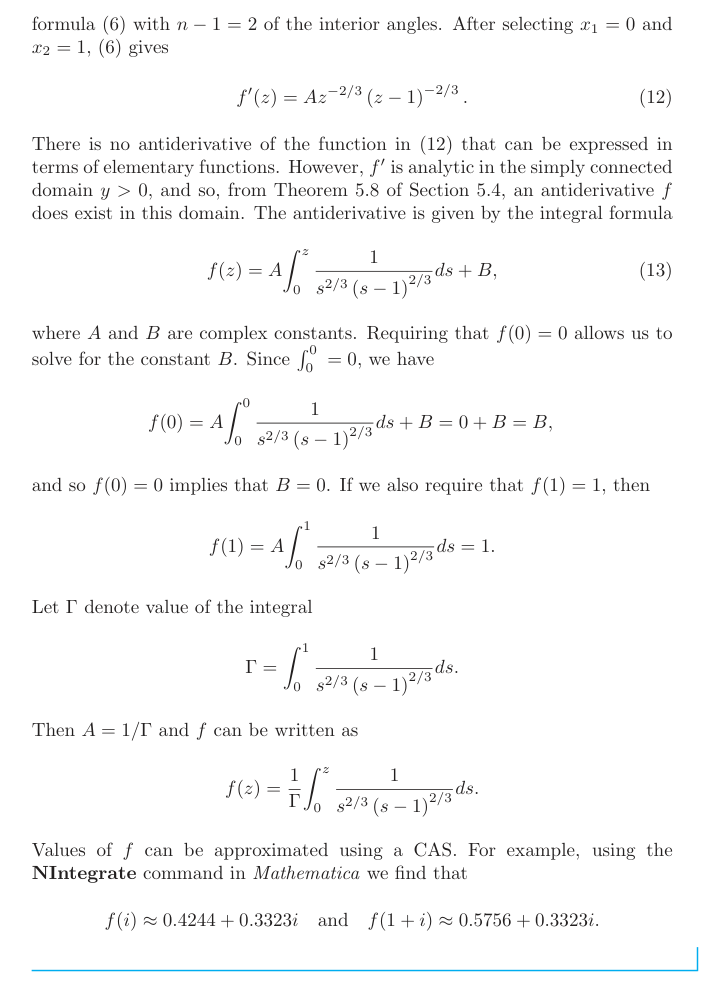
\includegraphics[width=\textwidth]{5-共形映射-2025061000.png}
% \caption{}
\label{}
\end{figure}
\begin{figure}[H]
\centering
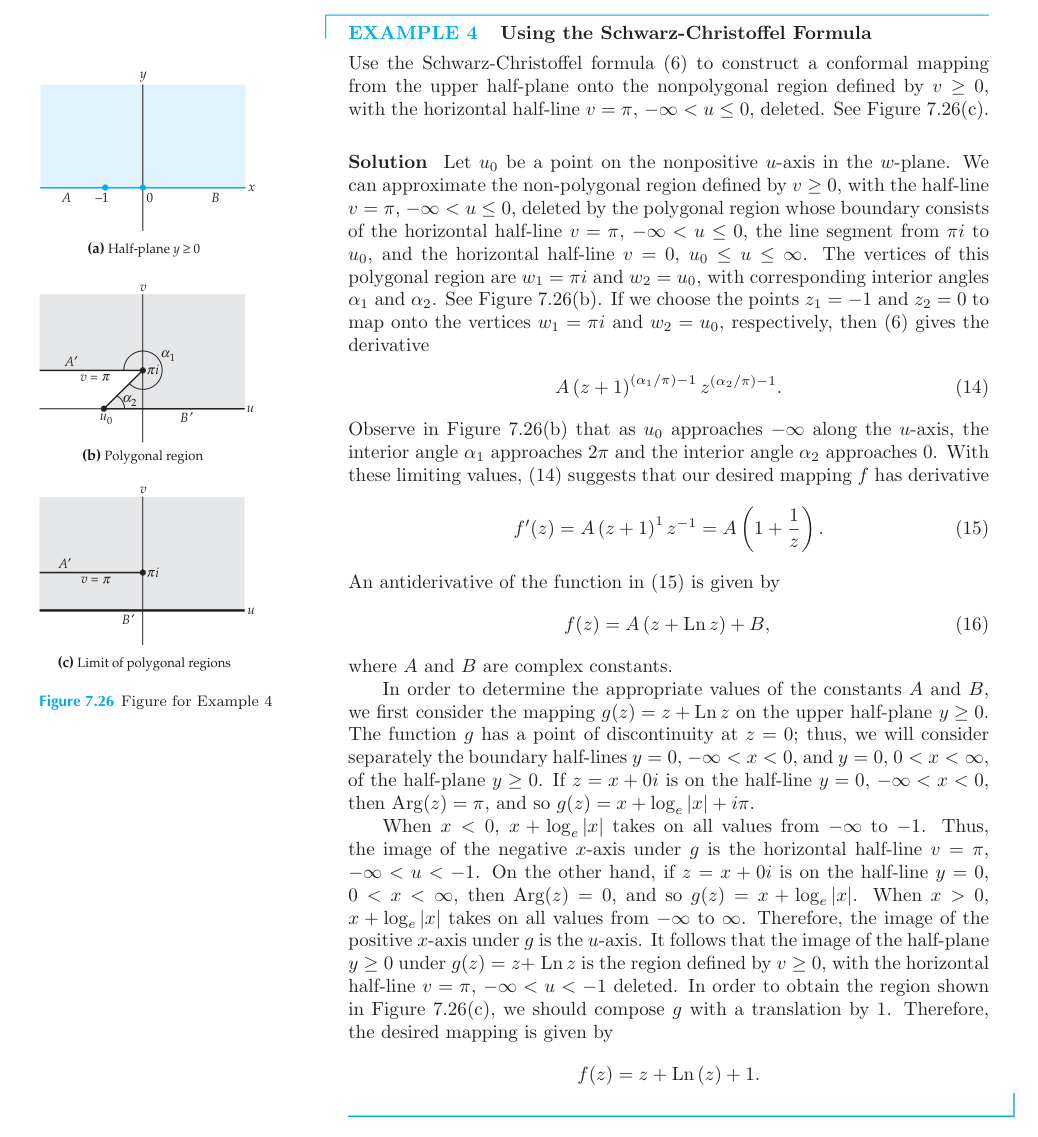
\includegraphics[width=\textwidth]{6-共形映射-2025061000.png}
% \caption{}
\label{}
\end{figure}

\subsection{Poisson Integral Formulas}

See Section 7.4....

\subsection{Applications}

See Section 7.5....

\subsection{映射 \texorpdfstring{$\frac{z-z_0}{1-\overline{z_0}z}$}{(z-z_0)/(1-overlinez_0z)}, \texorpdfstring{$\lvert z_0 \rvert<1$}{|z_0|<1}}

The expression $\frac{z-z_0}{1-\overline{z_0}z}$ has several important special properties in complex analysis, especially when $z_0$ is a point within the unit disk (i.e., $|z_0| < 1$). This expression is commonly known as a \textbf{Blaschke factor} (or a component thereof) and is also a type of \textbf{Möbius transformation}.

Here are some of its key properties:

\begin{enumerate}
	\item \textbf{Maps the unit disk to itself}: If $|z_0| < 1$, this transformation maps the open unit disk $D = \{z \in \mathbb{C} : |z| < 1\}$ to itself. That is, if $|z| < 1$, then $\left|\frac{z-z_0}{1-\overline{z_0}z}\right| < 1$.
	\item \textbf{Maps the unit circle to itself}: If $|z_0| < 1$, this transformation also maps the unit circle $C = \{z \in \mathbb{C} : |z| = 1\}$ to itself. That is, if $|z| = 1$, then $\left|\frac{z-z_0}{1-\overline{z_0}z}\right| = 1$.
	\item \textbf{Zero}: The transformation has a zero at $z = z_0$. That is, when $z = z_0$, $\frac{z_0-z_0}{1-\overline{z_0}z_0} = 0$.
	\item \textbf{Pole}: The transformation has a pole at $z = 1/\overline{z_0}$. If $|z_0| < 1$, then $1/|\overline{z_0}| = 1/|z_0| > 1$, so this pole lies outside the unit disk.
	\item \textbf{Conformal automorphism}: When $|z_0| < 1$, this expression (or when multiplied by a constant $e^{i\phi}$ with modulus 1) is a conformal automorphism of the unit disk onto itself (i.e., a biholomorphic map). This means it preserves angles and is a one-to-one and onto mapping.
	\item \textbf{Inverse Transformation}: If $f(z) = \frac{z-z_0}{1-\overline{z_0}z}$, its inverse transformation is $f^{-1}(w) = \frac{w+z_0}{1+w \overline{z_0}}$. This can be seen as a transformation of the same form, $f_{-z_0}(w)$, where the parameter $-z_0$ replaces $z_0$ and the sign in the denominator is adjusted (or more precisely, it is $\frac{w-(-z_0)}{1-w\overline{(-z_0)}}$ if we rewrite $1+w\overline{z_0}$ as $1-w(-\overline{z_0})$).
	\item \textbf{Derivative at $z_0$}: Let $\phi_{z_0}(z) = \frac{z-z_0}{1-\overline{z_0}z}$. Its derivative at $z=z_0$ is $\phi_{z_0}'(z_0) = \frac{1}{1-|z_0|^2}$. This property is relevant in contexts such as Schwarz's Lemma.
\end{enumerate}

In summary, this expression defines a very important complex transformation that plays a central role in the geometry and function theory of the unit disk. It allows for a standardized way to map any point $z_0$ inside the unit disk to the origin, while preserving the disk and its boundary, which is fundamental in many areas of complex analysis.

\subsection{例题}

\begin{exercise}
设 $D = \{z \in \mathbb{C} : |z| < 1\}$, 若 $f \in H(D) \cap C(\overline{D})$ 使得 $|f(z)| = 1, \forall z \in \partial D$, 求全部 $f$.
\end{exercise}
\begin{proof}
若 $f$ 在 $D$ 有无穷个零点, 则若零点在 $D$ 内部有聚点, 则解析函数唯一性告诉我们 $f \equiv 0$, 这不可能, 若这些零点的聚点只在 $D$ 边界, 那么 $f$ 在聚点处应该为 0, 这也不可能. 所以我们知道 $f$ 在 $D$ 只有有限个零点 $z_1, z_2, \cdots, z_n$, 这里 $\{z_i\}_{i=1}^n$ 允许有相同的项出现.

考虑无零点函数
\[
g(z) = \frac{f(z)}{\prod_{i=1}^n \frac{z - z_i}{1 - \overline{z_i}z}} \in H(D) \cap C(\overline{D}),
\]
显然 $|g(z)| = 1, \forall z \in \partial D$ 且 $\frac{1}{g(z)} \in H(D) \cap C(\overline{D})$. 故由最大模定理知 $|g(z)| \equiv 1, \forall z \in \overline{D}$. 因此我们知道 $g$ 为常数, 所以
\[
f(z) = c \prod_{i=1}^n \frac{z - z_i}{1 - \overline{z_i}z}, c \in \mathbb{C} \setminus \{0\}.
\]
\end{proof}

\section{Table of Conformal Mappings}

\subsection{初等映射}

\begin{figure}[H]
\centering
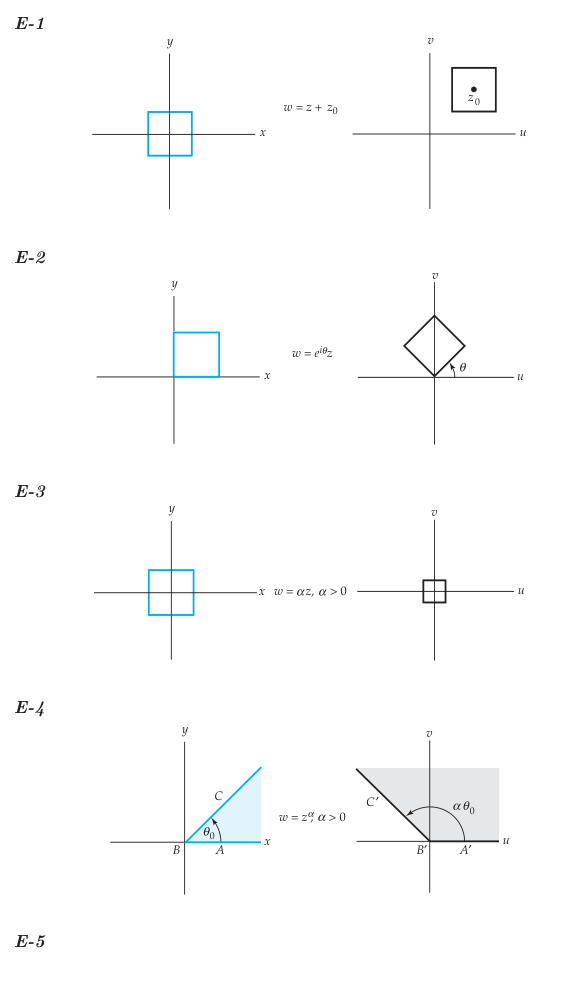
\includegraphics[width=\textwidth]{共形映射-2025061018.png}
% \caption{}
\label{}
\end{figure}
\begin{figure}[H]
\centering
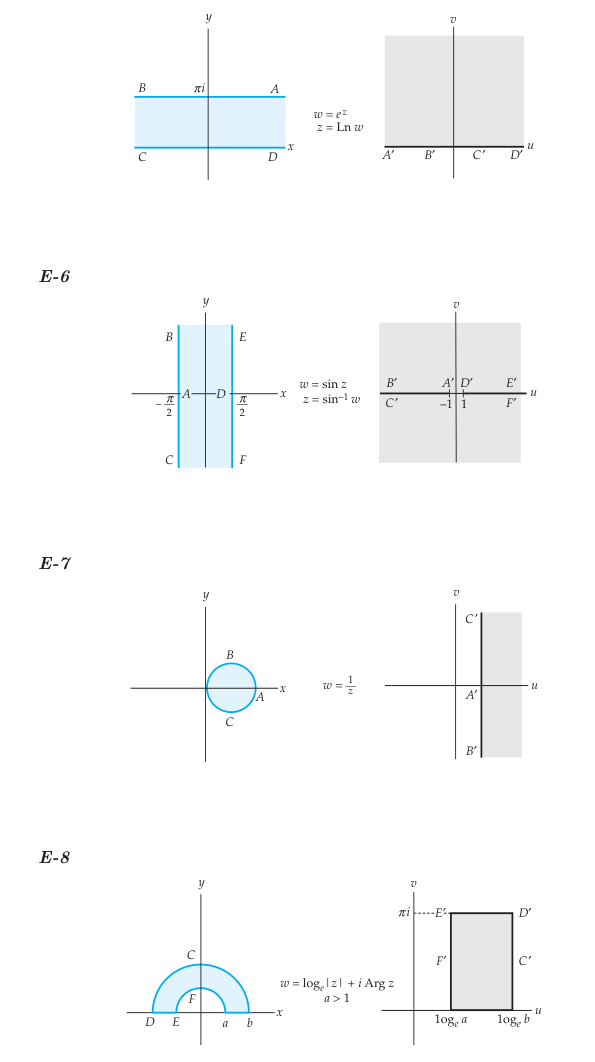
\includegraphics[width=\textwidth]{1-共形映射-2025061018.png}
% \caption{}
\label{}
\end{figure}

\begin{figure}[H]
\centering
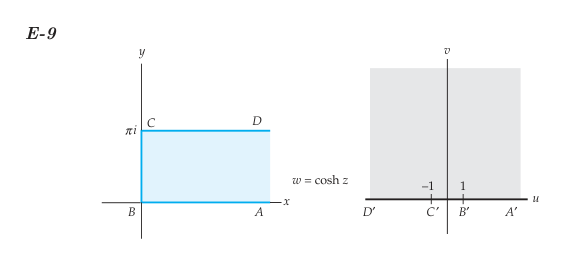
\includegraphics[width=\textwidth]{6-共形映射-2025061018.png}
% \caption{}
\label{}
\end{figure}

\subsection{Miscellaneous Mappings}

\begin{figure}[H]
\centering
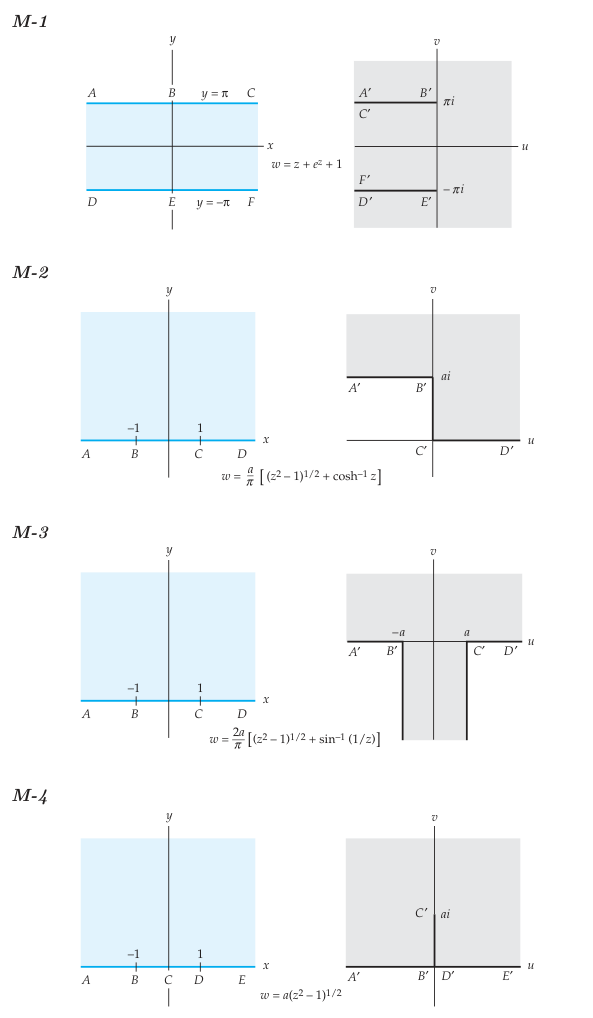
\includegraphics[width=\textwidth]{2-共形映射-2025061018.png}
% \caption{}
\label{}
\end{figure}
\begin{figure}[H]
\centering
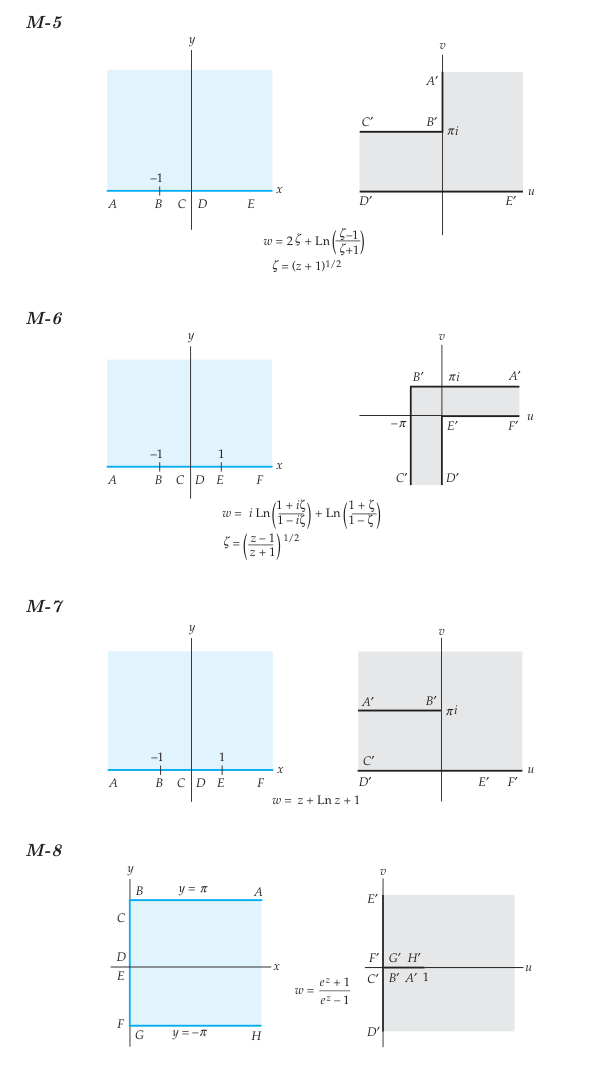
\includegraphics[width=\textwidth]{3-共形映射-2025061018.png}
% \caption{}
\label{}
\end{figure}
\begin{figure}[H]
\centering
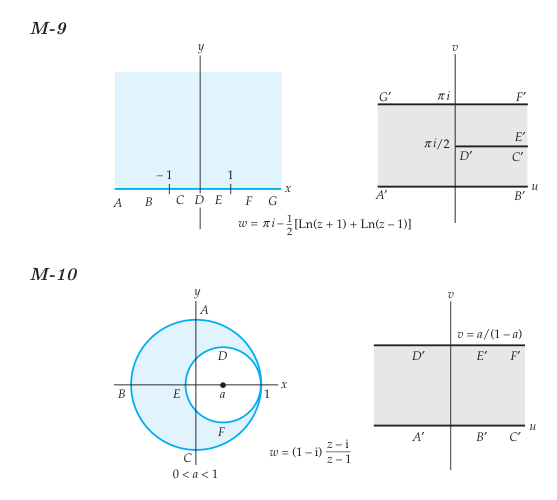
\includegraphics[width=\textwidth]{7-共形映射-2025061018.png}
% \caption{}
\label{}
\end{figure}

\subsection{Mappings to Circular Regions}

\begin{figure}[H]
\centering
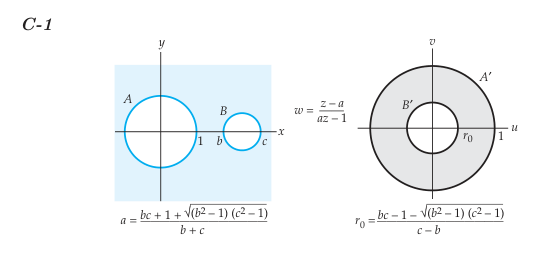
\includegraphics[width=\textwidth]{4-共形映射-2025061018.png}
% \caption{}
\label{}
\end{figure}
\begin{figure}[H]
\centering
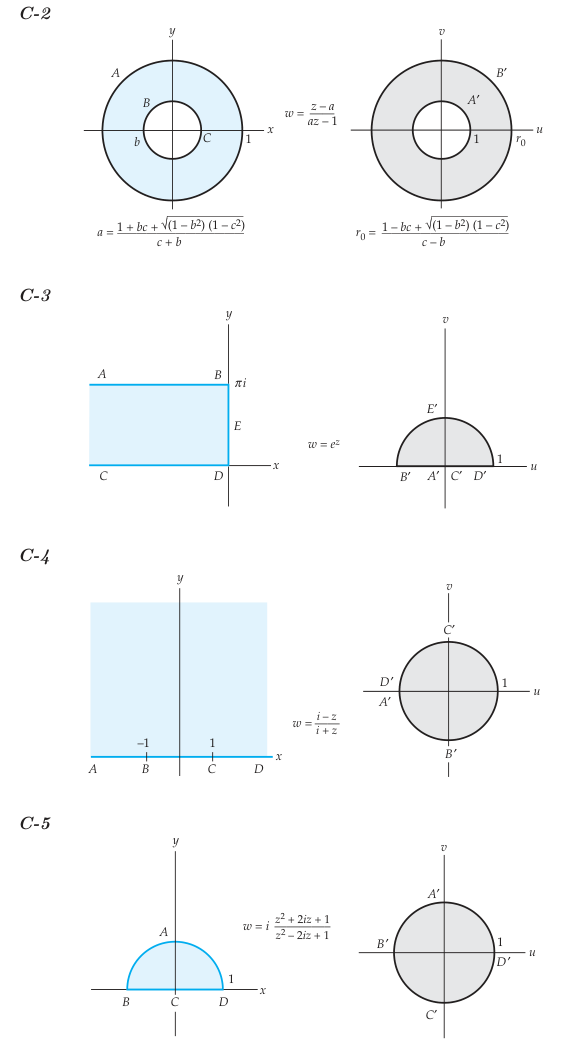
\includegraphics[width=\textwidth]{5-共形映射-2025061018.png}
% \caption{}
\label{}
\end{figure}

\subsection{Mappings of Half-Planes}

\begin{figure}[H]
\centering
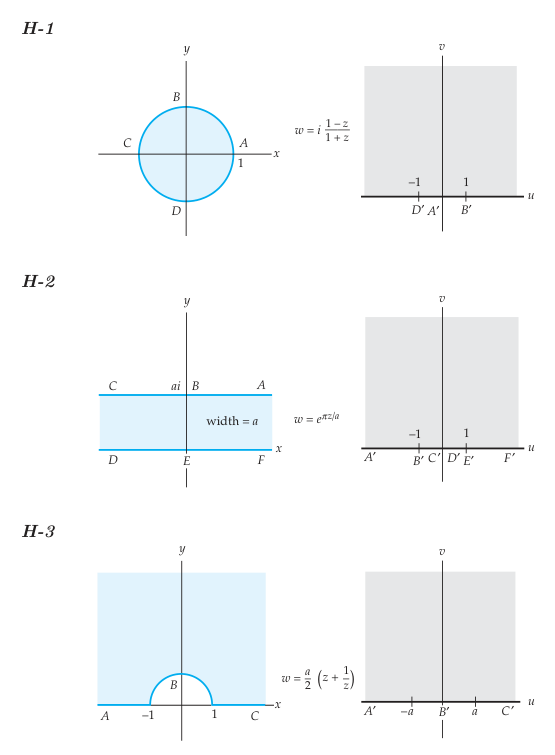
\includegraphics[width=\textwidth]{8-共形映射-2025061018.png}
% \caption{}
\label{}
\end{figure}
\begin{figure}[H]
\centering
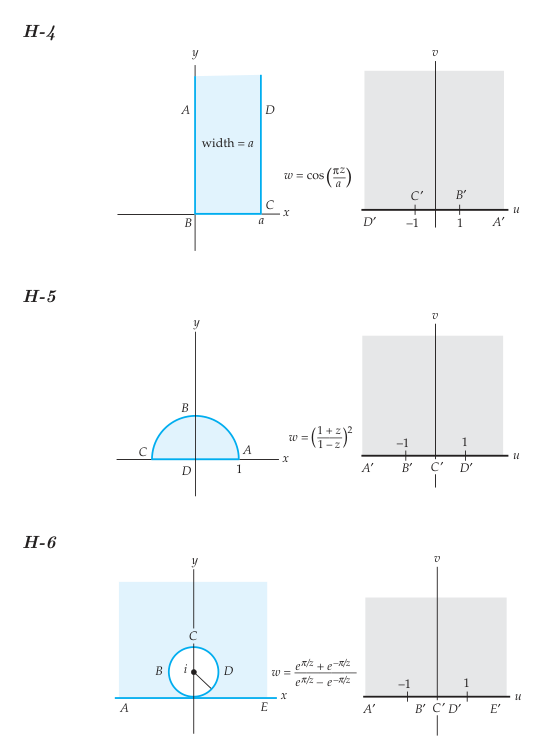
\includegraphics[width=\textwidth]{9-共形映射-2025061018.png}
% \caption{}
\label{}
\end{figure}
